\chapter{Übungsblatt 3}

\section{Aufgabe 1}

Was versteht man unter Relokation und Schutz? Welche Lösungsmöglichkeiten gibt
es?

Relokation ist das verschieben bzw umverteilen von pages. Hierfür werden die
Adressen entweder Dynamisch übersetzt oder sie werden beim Laden über den
Loader direkt überserzt.

Der Schutz stellt sichet, dass die Adressen nicht über den für das Programm
vorhergesehenen ADressbereich gehen. Wenn eine Adresse, welche über dem
Adressbereiches des Programms hinausgeht, aufgerufen wird, wird ein Fehler
gewrofen.

\section{Aufgabe 2}

Wie funktioniert das Verfahren der Speicherverwaltung mit Bitmaps? Wie
funktioniert das Verfahren der Speicherverwaltung mit einer verketteten Liste?
Vergleichen Sie die Verfahren. Gegeben sei folgende Speicherbelegung:

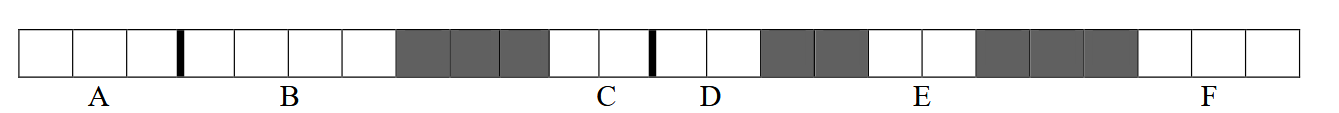
\includegraphics[width=\textwidth]{assets/uebungsblatt_3_task_2.png}

Das Verfahren mit einer Bitmap erzeugt eine Bitmap, welche die Bits mapt. Es
wird eine Liste generiert, wobei 1 angibt, dass die Speicherstellen belegt sind
und 0, dass die Speicherstelle frei ist.

\begin{tabular}{ | c | }
  1 1 1 1 1 1 1 0 0 0 1 1 1 1 0 0 1 1 0 0 0 1 1 1
\end{tabular}

[P, 3] -> [P, 4] -> [L, 3] -> [P, 2] -> [P, 2] -> [L, 2] -> [P, 2] -> [L, 3] -> [P, 3]

\section{Aufgabe 3}

Welche Algorithmen zur Speicherallozierung kennen Sie? Diskutieren Sie die Vor-
und Nachteile der Verfahren!

\section{Aufgabe 4}

Gegeben ist die folgende Adresse beim 4-stufigen Paging.

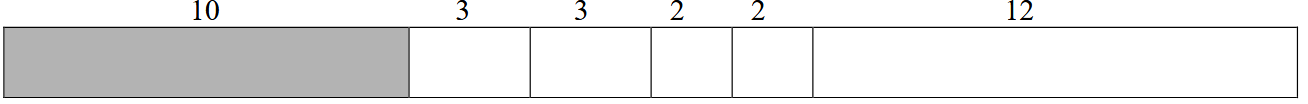
\includegraphics[width=\textwidth]{assets/uebungsblatt_3_task_4.png}

Zeichnen Sie ein Beispiel einer passenden Seitenrahmentabelle auf. Wie viele
Einträge können die einzelnen Tabellen enthalten? Erklären Sie das Verfahren
der Adressierung anhand der Adresse: 0000000000 101 001 10 00 100100100101.
Warum hat man mehrstufige Seitenrahmentabellen eingeführt? Welche Probleme
bringt dieses Verfahren mit sich? Wie kann man das 4-stufige Verfahren
beschleunigen?

\section{Aufgabe 5}

Gegeben sei ein Speicherbereich von einem GByte. Der Reihe nach kommen Anfragen
der Größe A=113 MB, B=43 MB, C=386 MB, D=96 MB an.

Zeichnen Sie das Prinzip der Speicherplatzvergabe nach dem Buddy-System anhand
der unten vorgegebenen Zeichnung auf.

\begin{tikzpicture}[
    font=\sffamily,
    every node/.style={font=\sffamily}
  ]

  \def\lineLength{8cm}
  \def\tickLabelOffset{1.5mm}
  \def\ySpacing{1.2cm}
  \def\xLineStart{3cm}
  \def\mainLabelXPos{\xLineStart - 0.5cm}

  \tikzset{
    custom diamond/.tip={Diamond[length=6pt, width=4.5pt, fill=black]}
  }

  \newcommand{\drawScale}[3]{
    \begin{scope}[yshift=-#1*\ySpacing]
      \node[anchor=east] at (\mainLabelXPos, 0) {#2=#3 MB};

      \coordinate (lineStart) at (\xLineStart, 0);
      \coordinate (lineEnd) at (\xLineStart + \lineLength, 0);

      \draw[-{custom diamond}] (lineStart) -- (lineEnd);
      \draw[{custom diamond}-{custom diamond}] (lineStart) -- (lineEnd);

      \node[below=\tickLabelOffset of lineStart, font=\small] {0};
      \node[below=\tickLabelOffset of lineEnd, font=\small] {1024};
    \end{scope}
  }

  \drawScale{0}{A}{113}
  \drawScale{1}{B}{43}
  \drawScale{2}{C}{386}
  \drawScale{3}{D}{96}

\end{tikzpicture}